\begin{frame}{Intersecciones y el problema MIS}
  
  Descripción:
  
  \begin{itemize}[<+->]
  \item Intersectar objetos geométricos en $\mathbb{R}^n$ suele
    ser un problema muy estudiado en Geometría Computacional.
    \begin{figure}  
      \centering
      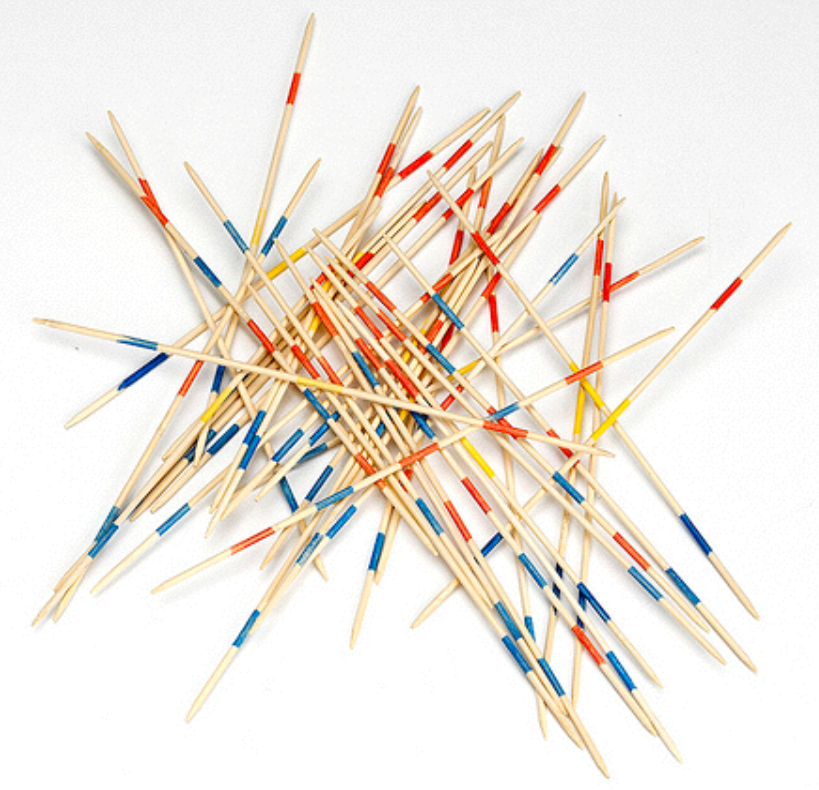
\includegraphics[width=0.25\textwidth]{./Images/Intersecciones.png}
    \end{figure}
    Podemos encontrar el número de intersecciones para segmentos en $\mathcal{O}(n \log n)$
    siendo sensible a su salida.
  \item ¿Podemos encontrar el máximo conjunto de objetos geométricos que no se intersecten?
  \item Encontrar el Conjunto Independiente Máximo (en adelante MIS) en una gráfica
    es uno de los problemas NP-Completo clásicos según Karp.
  \end{itemize}
\end{frame}

\begin{frame}{Colección de objetos geométricos.}
  
  Descripción:
  
  \begin{itemize}[<+->]
  \item Para una colección $\mathcal{L} = \{\ell_1, \dotsm, \ell_n\}$
    de objetos geométricos.
    \begin{figure}  
      \centering
      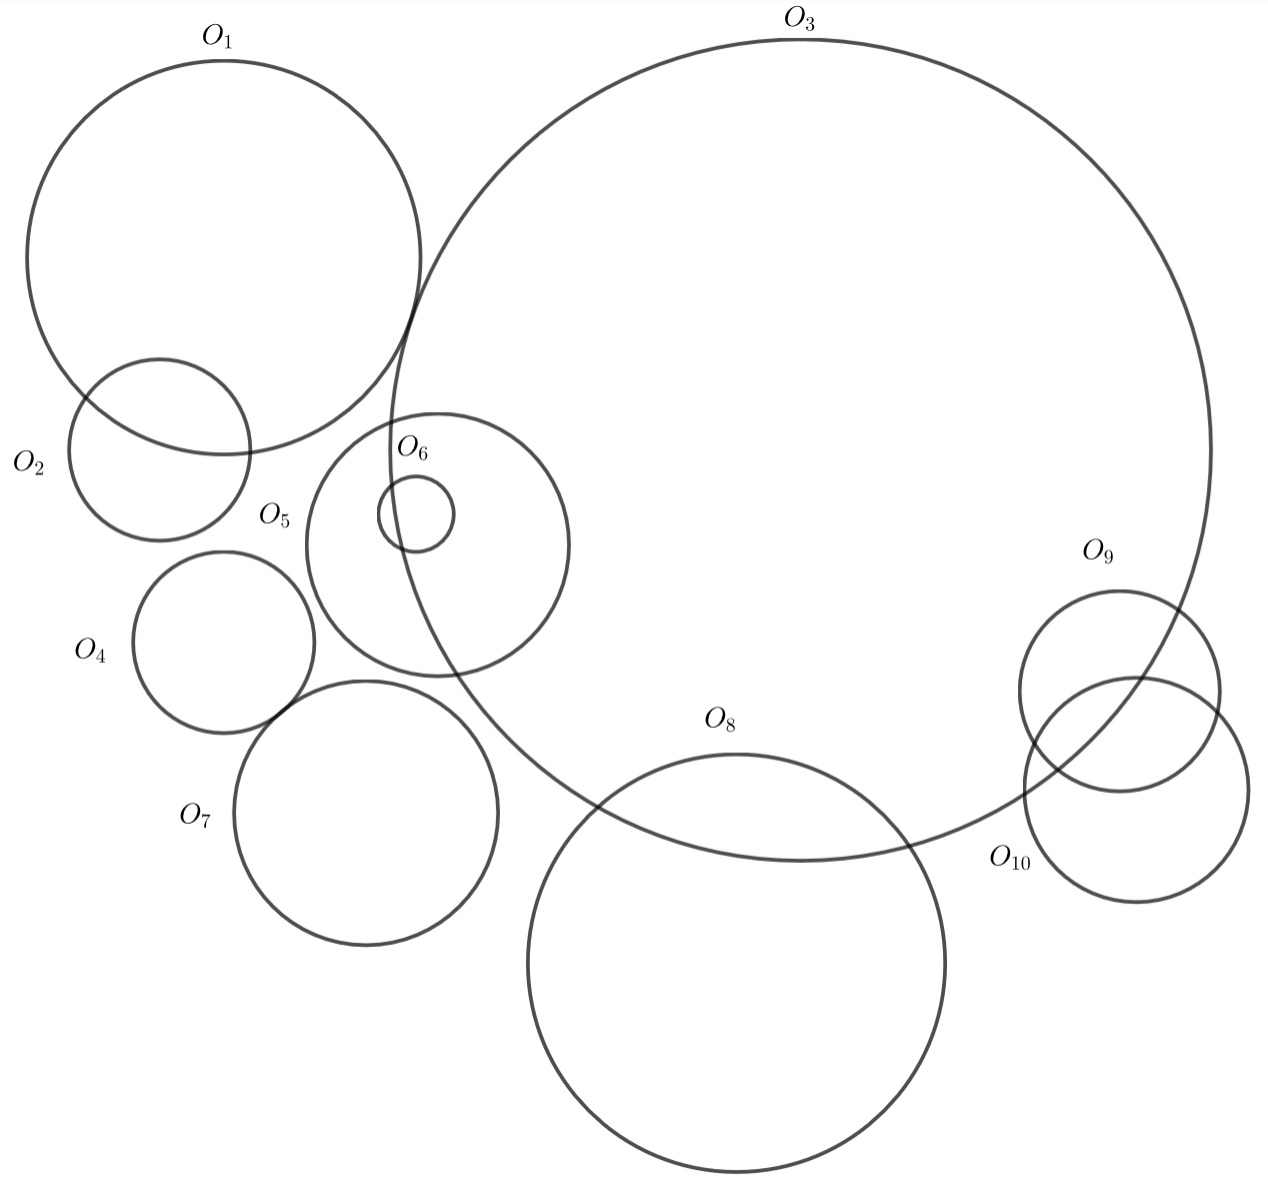
\includegraphics[width=0.7\textwidth]{./Images/Ejemplo01.png}
    \end{figure}
  \end{itemize}
\end{frame}

\begin{frame}{Dualidad.}
  
  \begin{itemize}[<+->]
  \item La gráfica de intersección $G_{\mathcal{L}} = (E_{\mathcal{L}},V_{\mathcal{L}})$
    de $\mathcal{L}$, cada objeto $\ell_i \in \mathcal{L}$ es representado por un vértice
    $v_i \in V_{\mathcal{L}}$ cualquier par $\ell_i \cap \ell_j \not= \varnothing$ se intersecta
    \textbf{SII} $(v_i, v_j) \in E_{\mathcal{L}}$.
    \begin{figure}  
      \centering
      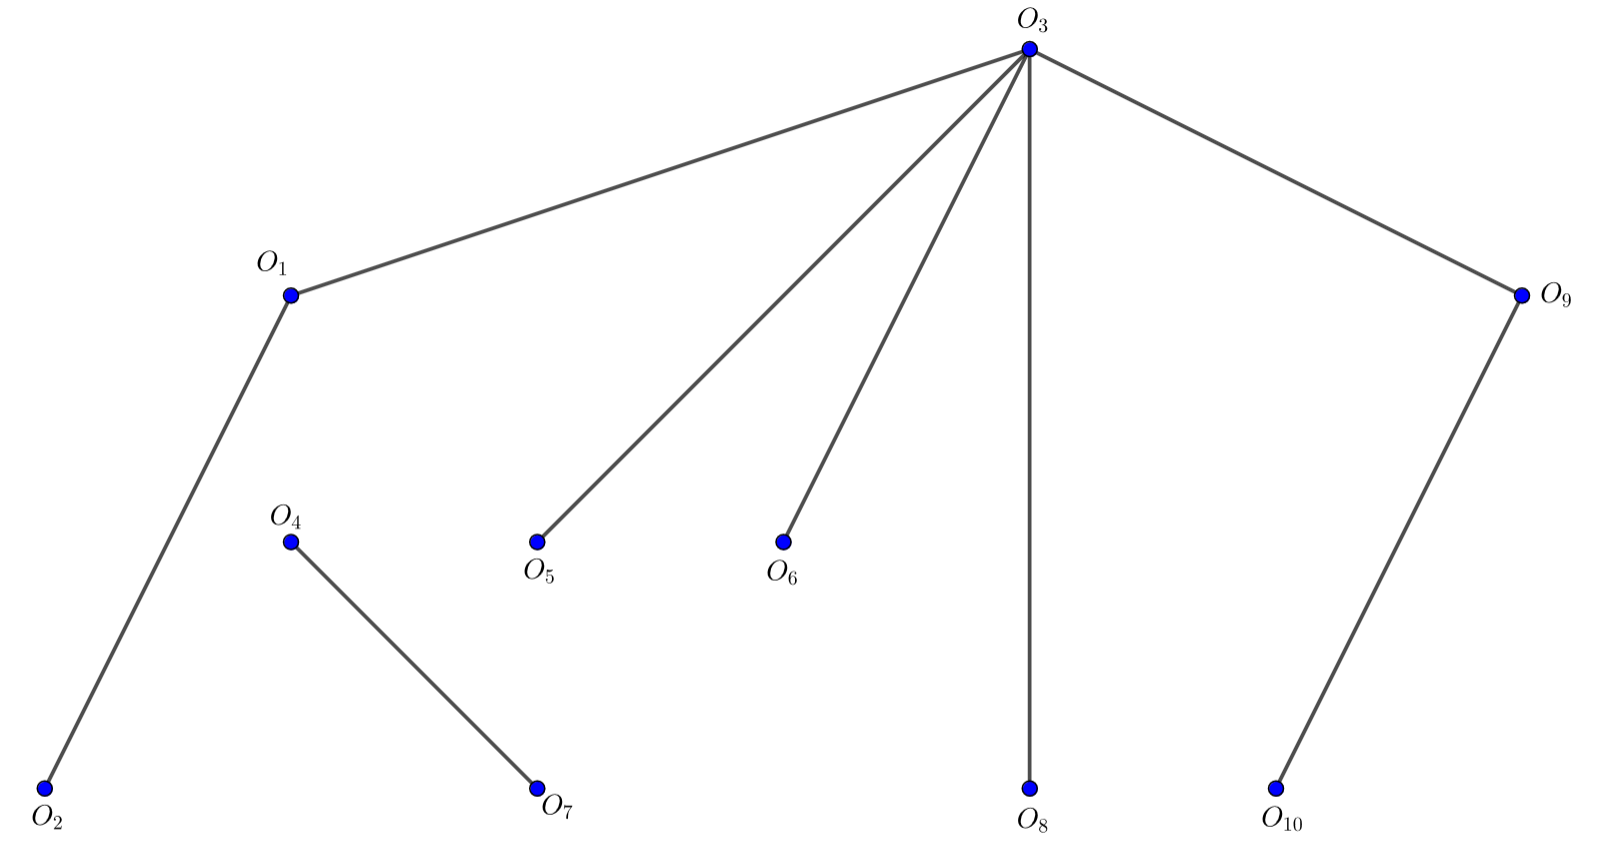
\includegraphics[width=0.8\textwidth]{./Images/Ejemplo02.png}
    \end{figure}
  \end{itemize}
\end{frame}

\begin{frame}{Conjuntos de discos independientes.}
  
  \begin{itemize}[<+->]
  \item Un conjunto independiente de $G_{\mathcal{L}}$ corresponde a un conjunto de objetos
    disjuntos por pares en $\mathcal{L}$.
    \begin{figure}  
      \centering
      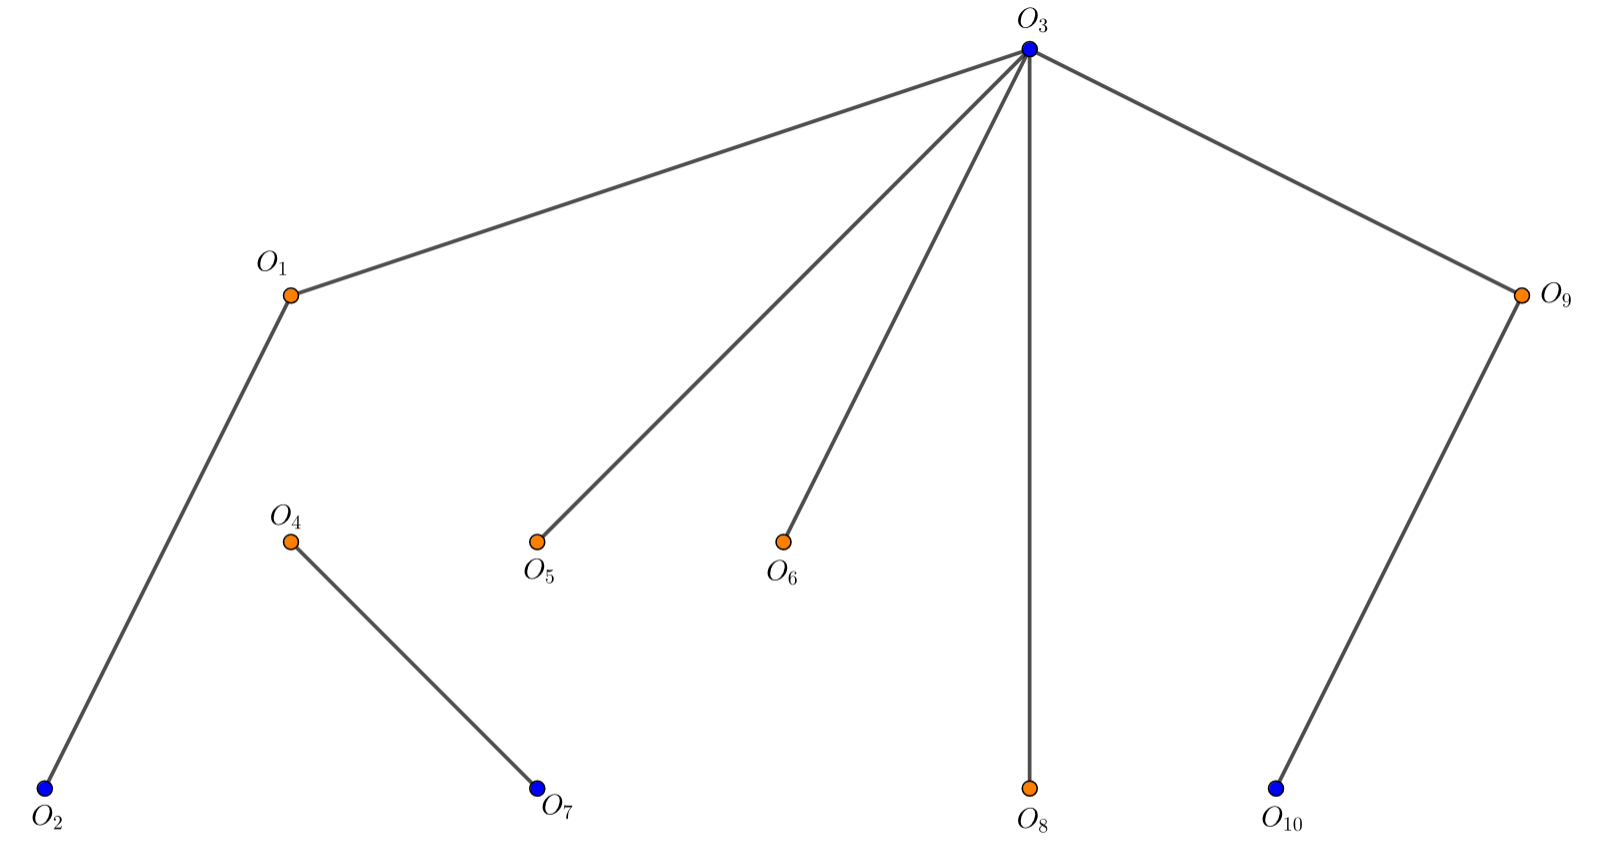
\includegraphics[width=0.8\textwidth]{./Images/Ejemplo03.png}
    \end{figure}
  \item Nuestro objetivo es mantener una estructura de datos que pueda mantener
    eficientemente un conjunto independiente $S \subseteq L$ cuyo tamaño sea una aproximación
    de factor constante del MIS de L en cualquier momento, con tiempos de actualización
    polilogarítmicos para inserciones y eliminaciones.
  \end{itemize}
  
\end{frame}


\begin{frame}{Antecedentes}
  
  Antecedentes:
  
  \begin{itemize}[<+->]
  \item En el 2022 Jean Cardinal et. al. crean el algoritmo \textit{offline} MIX para aproximar
    el conjunto independiente máximo de objetos gruesos en $\mathbb{R}^d$ con
    $d \in o(1)$ que se ejecuta en tiempo $\mathcal{O}(\alpha \log \alpha)$ con
    $\alpha$ el valor del máximo candidato a solución (en adelante OPT).
  \item La función MIX utiliza dos estructuras de datos, una de reciente creación
    llamada \textit{Estructura del vecino más cercano/lejano}, que se bassa en la
    idea del diagrama de Voronoi.
  \item Chan et. al. logran generalizar la estructura anterior a dimensiones superiores, siempre
    que sean constante respecto al número de objetos geométricos.
  \end{itemize}
\end{frame}
